\section{Common Topologies} 

  We have given some examples of how we can construct topologies from scratch given an arbitrary set $X$, possibly with some structure. Now given a collection of 1 or more topological spaces, we will talk about how we can construct new topologies. Note that the topologies introduced in this section don't really require us to talk about functions yet. They can be constructed and completely described in terms of sets. 

\subsection{Orderings and the Dictionary Topology}

  \begin{definition}[Dictionary Topology]
    Let $X$ be a set with a simple order relation. Let $\B$ be the collection of all sets of the following types. 
    \begin{enumerate}
      \item All open intervals $(a, b) \subset X$
      \item All half-open intervals $[a_0, b)$, where $a_0$ is the minimum element of $X$
      \item All half-open intervals $(a, b_0]$, where $b_0$ is the maximum element of $X$. 
    \end{enumerate}
    This set $\B$ is a basis for the \textbf{order topology} of $X$. If $X$ has no minimum or maximum, then there are no sets of type of 2 or 3, respectively. 
  \end{definition}

  \begin{example}[Standard Order Topology on $\mathbb{R}$]
    The standard topology on $\mathbb{R}$ is precisely the order topology derived from the usual order on $\mathbb{R}$. Since $\mathbb{R}$ has no minimum or maximum, the basis consists of open intervals $(a, b) \subset \mathbb{R}$ with $a, b \in \mathbb{R}$. 
  \end{example}

  \begin{example}[Basis of Open Intervals with Rational Endpoints]
    We can however get away with smaller basis that generate the same topology on $\mathbb{R}$. If we take the set of all open intervals $(a, b) \subset \mathbb{R}$ with $a, b \in \mathbb{Q}$, this is also a basis for the same standard order topology. Too see why, let us denote this basis as $\B^\prime$ and the basis of all open intervals with real endpoints be $\B$. Then, clearly $B^\prime \subset \B \implies \T^\prime \subset \T$. As for the other, way, let us take an open interval $(a, b) \in \B$. Then we can see that 
    \begin{equation}
      (a, b) = \bigcup_{\substack{p, q \in \mathbb{Q} \\ a < p, q < b}} (p, q)
    \end{equation}
    where equality follows from density of rationals in $\mathbb{R}$. 
  \end{example}

  \begin{example}[$\mathbb{R}^2$ with Dictionary Order]
    Given $\mathbb{R} \times \mathbb{R}$ with the dictionary order, then $\mathbb{R} \times \mathbb{R}$ has neither a largest nor smallest element. Therefore, the order topology on $\mathbb{R} \times \mathbb{R}$ consists of all "intervals" of form
    \begin{equation}
      \big((a, b), (c, d) \big) \equiv  \{(x, y) \in \mathbb{R}^2 \mid (a, b) < (x, y) < (c, d)\}
    \end{equation}

    \begin{figure}[H]
      \centering 
      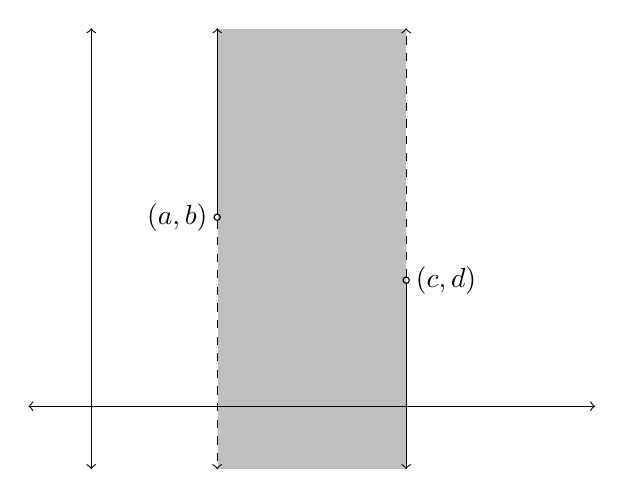
\begin{tikzpicture}[scale=0.8]
        \draw[white, fill=lightgray] (2,-1) rectangle (5,6);
        \draw[<->] (-1,0)--(8,0);
        \draw[<->] (0,-1)--(0,6);
        \draw[->] (2,3.05)--(2,6);
        \draw[->] (5,1.95)--(5,-1);
        \draw (2,3) circle [radius=0.05];
        \draw (5,2) circle [radius=0.05];
        \draw[dashed, ->] (2,2.95)--(2,-1);
        \draw[dashed,->] (5,2.05)--(5,6);
        \node[left] at (2,3) {$(a, b)$};
        \node[right] at (5,2) {$(c,d)$};
      \end{tikzpicture}
      \caption{This means that open rays and lines are also a part of the topology of $\mathbb{R} \times \mathbb{R}$. } 
      \label{fig:r2_dict_order}
    \end{figure}
  \end{example}

  \begin{example}[Positive Integers]
    The set of positive integers $\mathbb{Z}_+$ form an ordered set with a smallest element. The order topology for $\mathbb{Z}_+$ is precisely the discrete topology since every one-point set is an open set. 
    \begin{equation}
      \{n\} = (n-1, n+1)
    \end{equation}
  \end{example}

  \begin{example}[Two Copies of Positive Integers]
    The dictionary order topology on $\{1, 2\} \times \mathbb{Z}_+$ results in every one point set being open, except for the point $(2, 1)$. Since every neighborhood of $(2,1)$ must contain some point of form $(1, n)$ for arbitrarily large $n$, $\{(2,1)\}$ is not open. 
  \end{example}

  \begin{definition}
    If $X$ is an ordered set a $a \in X$, then there are 4 subsets of $X$ called rays determined by $a$. 
    \begin{enumerate}
      \item $(a, +\infty)$ 
      \item $(-\infty, a)$
      \item $[a, +\infty)$
      \item $(-\infty, a]$
    \end{enumerate}
    The first two sets are called \textbf{open rays}, and the latter two sets are called \textbf{closed rays}. 
  \end{definition}

  We can extend the basis of open intervals to some other basis based on the order, which generates other topologies. 

  \begin{example}[Lower/Upper Limit Topology]
    Given a totally ordered set $(X, \leq)$, 
    \begin{enumerate}
      \item the \textbf{lower limit topology} is the topology generated by the basis of all half-closed half-open intervals of form 
      \begin{equation}
        [a, b) \coloneqq \{ x \in X \mid a \leq x < b \}
      \end{equation}
      \item the \textbf{upper limit topology} is the topology generated by the basis of all half-open half-closed intervals of form 
      \begin{equation}
        (a, b] \coloneqq \{ x \in X \mid a < x \leq b \}
      \end{equation}
    \end{enumerate}
  \end{example}

  \begin{example}[Nested Interval Topology]
    In the space $X = (0,1)$, the \textbf{nested interval topology} is the topology generated by the basis of nested intervals of the form 
    \begin{equation}
      \B_{ni} \coloneqq \{ (0, 1-\frac{1}{n}) \mid n \in \mathbb{N} \}
    \end{equation}
  \end{example}

  A topology generated by closed intervals can also be a topology! 

  \begin{example}[Closed Interval Topology]
    In the set $X = [-1, 1]$, the following set 
    \begin{equation}
      \B_{ci} \coloneqq \{ [-1, a) \mid a > 0 \big\} \bigcup \big\{ (b, 1] \mid b<0 \}
    \end{equation}
    is a basis. The topology it generates is called the \textbf{closed interval topology}, denoted $\T_{ci}$. 
  \end{example}

  Finally, we talk about a seemingly arbitrary topology called the K-topology, but it is useful for counterexamples.   

  \begin{example}[K-Topology]
    In $\mathbb{R}$, let us denote $K = \{1/n\}_{n \in \mathbb{N}}$. Then the \textbf{K-topology} on $\mathbb{R}$ is the topology generated by the basis consisting of 
    \begin{enumerate}
      \item all open intervals $(a, b)$ with $a, b \in \mathbb{R}$. 
      \item all sets of the form $(a, b) \setminus K$ with $a, b \in \mathbb{R}$. 
    \end{enumerate}
  \end{example} 

  Now that we have some collection of topologies, let's try to compare them. We claim the following. 

  \begin{theorem}[Comparison of Topologies of the Real Line]
    
  \end{theorem}

\subsection{Metric Topology}

  For common sets like $\mathbb{R}^n$, which has an inner product, or $\mathbb{Q}$, which has an order, it is easy to build these topologies with set-builder notation. Consider the following. 

  \begin{definition}[Metric Topology]
    Given a metric space $(X, d)$, let us denote the \textbf{metric topology}, or \textbf{open-ball topology}, as the set of subsets $U$ satisfying the property that for all $x \in U$, there exists a positive $r \in \mathbb{R}$ such that $B(x, r) \subset U$, where $B(x, r) \coloneqq \{y \in X \mid d(x, y) < r\}$ is the open ball of radius $r$ around $x$. We claim that this is a topology. 
  \end{definition} 
  \begin{proof}
    We show that the properties of a topology hold. 
    \begin{enumerate} 
      \item For the empty set, the inclusion of an open ball for a point in $\emptyset$ is vacuously satisfied. For the whole set, we choose any point $x$ and any $r$, and the open ball is trivially a subset of $X$. 

      \item Let $\{U_\alpha\}_{\alpha \in I}$ be a collection of open subsets of $X$. Let their union be denoted $U$. We claim $U$ is open. Pick any point $x \in U$. Then by definition of union, there exists some $\alpha \in I$ s.t. $x \in U_\alpha$. Since $U_\alpha$ is open, there exists a $r > 0$ s.t. $B(x, r) \subset U_\alpha \subset U$. Therefore $U$ is open. 

      \item Let $U_1, \ldots, U_k$ be open, and let us denote their intersection as $U$. We claim $U$ is open. Pick a point $x \in U$. Then for each $i = 1, \ldots, k$, $x \in U_i$ and there exists a corresponding $r_i > 0$  such that the open ball $B(x, r_i) \subset U_i$. Take the set $R = \{r_i\}$, which is a finite set living in $\mathbb{R}$. We will take for granted that every finite subset of an ordered set has a minimum.\footnote{If we wish to prove it, we can start with a singleton set, claim that its minimum is the only element. Then we use induction by assuming for a set $R$ of size $k$ that a minimum exists, and by adding $1$ more element $r$ we update the minimum to be $\min\{r, \min{R}\}$ and show that this is indeed the minimum.} Let us denote $r^\ast = \min{R}$, and we claim that $r^\ast$ gives us a ball that can fit inside $U$. Assume $y \in B(x, r^\ast)$. Then 
      \begin{align}
        y \in B(x, r^\ast) & \implies d(x, y) < r^\ast \\ 
                           & \implies d(x, y) < \min{R} \\
                           & \implies d(x, y) < r_i \text{ for } i = 1, \ldots, k \\
                           & \implies y \in B(x, r_i) \text{ for } i = 1, \ldots, k
      \end{align} 
      Since $B(x, r_i)$ by construction is contained within $U_i$, $y \in U_i$ for all $i$. This means by definition of intersection that $y \in U$, and we have proven that $B(x, r^\ast)$ completely fits inside $U$. 
    \end{enumerate}
  \end{proof} 

  Note that while open balls are used to define whether a set is open or not, the definition doesn't state whether open balls themselves are open sets. It turns out that it is easy to prove that they are. 
  
  \begin{lemma}[Open Balls are Open Sets]
    The open ball wrt any metric $d$ is an open set wrt the metric topology. 
  \end{lemma}
  \begin{proof}
    Let $y \in B(x, r)$. Then $d(x, y) < r \implies 0 < r - d(x, y)$. To show that $B(x, r)$ is open, we would like to show that there exists some $r^\prime > 0$ s.t. $y \in B(y, r^\prime) \subset B(x, r)$. Set $r^\prime = r - d(x, y)$. Then 
    \begin{align}
      z \in B(y, r^\prime) & \implies d(y, z) < r - d(x, y) \\
                           & \implies d(x, y) + d(x, y) < r \\
                           & \implies d(x, z) < r \\
                           & \implies z \in B(x, r)
    \end{align} 
    and so $B(y, r^\prime) \subset B(x, r)$. We are done. 
  \end{proof}

  \begin{example}[Discrete Metric Induces Discrete Topology]
    Given a set $X$, induce the metric $d$ defined
    \begin{equation}
      d(x, y) \equiv \begin{cases} 1 & \text{if } x \neq y \\ 0 & \text{if } x = y \end{cases}
    \end{equation}
    This metric induces the discrete topology on $X$, since the basis elements of the open balls
    \begin{equation}
      B_r (x) \equiv \{ y \in X \mid d(x, y) <r\}
    \end{equation}
    consists of two types of open sets. When $r \leq 1$, then $B_r (x) = x$ (since the radius is $0$). If $r > 1$, then the open set is the entire space $X$. 
  \end{example} 

  While the behavior for finite sets are predictable under the metric topology, as soon we we get into infinite sets, the properties of the metric topology may differ. 

  \begin{example}[Metric Topologies on $\mathbb{Z}$ and $\mathbb{Q}$]
    $\mathbb{Z}$ and $\mathbb{Q}$ are countable sets, so there is a bijection between them. If we give each of them the metric topology, $\mathbb{Z}$ ends up having the discrete topology (take the $0.5$-ball around each integer), whereas for $\mathbb{Q}$, we will see later that by the density of the rationals there are an infinite number of rationals in $(q - r, q + r)$ for $q \in \mathbb{Q}$. Therefore, the metric topology may or may not induce the discrete topology. 
  \end{example}

  \begin{example}[Supremum Norm in $\mathbb{R}^3$]
    \begin{figure}[H]
      \centering 
      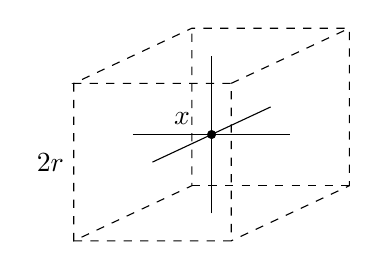
\begin{tikzpicture}
        \draw[dashed] (0,0)--(2,0)--(2,2)--(0,2)--(1.5,2.7)--(3.5,2.7)--(3.5,0.7)--(2,0);
        \draw[dashed] (2,2)--(3.5,2.7);
        \draw[dashed] (0,2)--(0,0)--(1.5,0.7)--(1.5,2.7);
        \draw[dashed] (1.5,0.7)--(3.5,0.7);
        \draw (1,1)--(2.5,1.7);
        \draw (0.75,1.35)--(2.75,1.35);
        \draw (1.75,0.35)--(1.75,2.35);
        \draw[fill] (1.75,1.35) circle (0.05);
        \node[above left] at (1.6,1.35) {$x$};
        \node[left] at (0,1) {$2r$};
      \end{tikzpicture}
      \caption{In $\mathbb{R}^3$, each basis element is a cube centered at $x$ with side lengths $2r$.} 
      \label{fig:}
    \end{figure}
  \end{example}

  \begin{theorem}[Metric Topologies on Finite Sets]
    If $(X, d)$ is a finite metric space, then the metric topology on it is the discrete topology. 
  \end{theorem}
  \begin{proof}
    Take all pairwise points and compute $\epsilon = \min_{x \neq y} \{d(x, y)\}$. Since $X$ is finite, all pairs are finite and therefore the minimum exists. Now let us take the $\epsilon$-ball around $x$. Then every $y \neq x$ has distance $d(x, y) \geq \epsilon$, and therefore $y \not\in B(x, \epsilon)$. So all single points are open sets, which induces the discrete topology. 
  \end{proof}

  It is easy to go from a metric to a topology, but a natural question is that given a topology, does there exist a metric that induces this topology? This is precisely the notion of \textit{metrizability}, which is a highly desirable attribute for spaces, and there are many existence theorems that proves metrizability given certain conditions.

  \begin{definition}[Metrizable Space]
    If $(X, \T)$ is a topological space, $(X, \T)$ is said to be \textbf{metrizable} if there exists a metric $d$ on $X$ that induces the topology $\T$ of $X$.
  \end{definition}

  \begin{example}[Non-Metrizable Finite Spaces]
    Let $X = \{a, b c\}$. Then the topology 
    \begin{equation}
      \T = \{\emptyset, \{b\}, \{a, b\}, \{b, c\}, X \}
    \end{equation} 
    is not metrizable from the theorem above since the only metrizable topologies are discrete. 
  \end{example}

  \begin{lemma}[Fineness of Metric Topologies]
    Let $d$ and $d^\prime$ be two metrics on the set $X$ with their respective induced topologies $\T, \T^\prime$. We claim that $\T \subset \T^\prime$ iff there exists a $M > 0$ s.t. 
    \begin{equation}
      d^\prime (x, y) < M \cdot d(x, y)
    \end{equation} 
    for all $x, y \in X$. That is, we can bound $d^\prime$ with a constant multiple of $d$. 
  \end{lemma}
  \begin{proof}
    
  \end{proof}

\subsection{Euclidean Topology}

  More specifically, the metric topology generated by the $L_2$-metric on $\mathbb{R}^n$ is called the \textbf{Euclidean topology}. Note that the topological property of stability under countable intersection was required to show that the minimum of $R$ existed. This is not true for infinite sets in general. This gives us some motivation as to why we need the \textit{finite} intersection rather than an infinite one. 
  
  \begin{lemma}[Singletons are Not Open in $\mathbb{R}^n$]
    A singleton set is not open in $\mathbb{R}^n$ with the Euclidean topology.   
  \end{lemma}
  \begin{proof}
    We claim that the singleton set $S = \{0\}$ is not open under the Euclidean metric. We pick a point in $S$, which can only be $0$. Assume that there exists an $r > 0$ s.t. $B(x, r) \subset S$. $\mathbb{R}$ is Archimedean, so there exists a natural number $N$ s.t. $0 < 1/N < r$. We construct the vector $v = (v_1, \ldots, v_n)$ s.t. $v_1 = 1/N$ and $v_i = 0$ everywhere else. The distance between $0$ and $v$ is 
    \begin{equation}
      \| v - 0 \| = \|v\| = \sqrt{(1/N)^2} = 1/N < r
    \end{equation} 
    so $v \in B(x, r)$. But $v \neq 0$, and by contradiction such an $r$ cannot exist. In $\mathbb{R}^n$ we consider the countable intersection of open balls (which we have proved in class are open sets) around $0$ of radius $1/N$ for $n \in \mathbb{N}$. We claim that 
    \begin{equation}
      \bigcap_{n \in \mathbb{N}} B(0, 1/n) = \{0\}
    \end{equation} 
    We see that $1/n$ must always be positive and so $\|0 - 0\| = 0 < 1/n$. Therefore the LHS $\supset $ RHS. To see that the intersection contains no other element, consider any vector $v \neq 0$. Then by definition of the metric, $d(v, 0) > 0$. By the Archimedean property, there exists a natural $N \in \mathbb{N}$ s.t. $0 < 1/N < d(v, 0)$, which means that $v \not\in B(0, 1/N)$, and so $v$ cannot be in the intersection. Therefore, the intersection must be $\{0\}$, and we have shown that $B_0$ is not open, so we are done. 
  \end{proof}

  \begin{theorem}
    For a metric space $(X, d)$, the metric topology is finer than the cofinite topology. 
  \end{theorem} 
  \begin{proof}
    Note that if $X$ is finite, then both are reduced to the discrete topologies. 
  \end{proof}

  While it is not surprising that a basis uniquely generates a topology, it is not immediately obvious \textit{what} the generated topology looks like. It turns out that many different bases may generate the same topology, and the concept of fineness allows us to compare these topologies more effectively. For example, if two topologies are both finer than the other, then they must be equal. 

  \begin{theorem}[Euclidean Topology on $\mathbb{R}^n$]
    $L_p$ norms all generate the same topology on $\mathbb{R}^n$. 
  \end{theorem}
  \begin{proof}
    We can show that 
    \begin{equation}
      n^q d_\infty \leq n^q d_2 \leq n^q d_1 \leq d_p \leq n^{-p} d_\infty
    \end{equation}
    where $q$ is the holder conjugate of $p$. Visually, we can see that every open ball in $(\mathbb{R}^n, d)$ (with the Euclidean metric) is the form to the left, while an open ball in $(\mathbb{R}^n, \rho)$ (with the square metric) is of form on the right. 
    \begin{center}
      \begin{tikzpicture}[scale=0.5]
        \draw [dashed] (1,0) circle [radius=2];
        \draw [dashed] (6,-2) rectangle (10,2);
        \draw [fill] (1,0) circle [radius=0.05];
        \node [above left] at (1,0) {x};
        \draw (1,0)--(3,0);
        \node [above] at (1.5,0) {r};
        \draw [fill] (8,0) circle [radius=0.05];
        \node [below right] at (8,0) {x};
        \draw (8,0)--(10,0);
        \draw (8,0)--(8,2);
        \node [right] at (8,1) {r};
        \node [above] at (9,0) {r};
      \end{tikzpicture}
    \end{center}
    Clearly, we can form any open set of any "shape" using any arbitrary combination of these "circles" or "squares," indicating that they generate the same topology. 
  \end{proof}

\subsection{Cofinite Topology}

  \begin{definition}[Cofinite Topology]
    Given a set $X$, the set of all subsets $U$, satisfying the property that $X \setminus U$ is finite, is a topology, called the \textbf{cofinite topology} or the \textbf{finite complement topology}.\footnote{While this definition may seem a bit arbitrary, this is very similar to the Zariski topology, which is used in algebraic topology.} 
  \end{definition}
  \begin{proof}
    Let us denote this set $\T_c$. 
    \begin{enumerate}
      \item By definition $\emptyset \in \T_c$. It is clear that $X \setminus X = \emptyset$ has cardinality $0$, and therefore is in $\T_c$. 

      \item Let $\{U_\alpha\}_{\alpha \in I} \in \mathcal{T}_c$ by a collection of open sets of $X$. Then by deMorgan's laws, 
      \begin{equation}
        X \setminus \bigcup_{\alpha \in I} U_{\alpha} = \bigcap_{\alpha \in I} (X \setminus U_\alpha)
      \end{equation}
      $X \setminus U_\alpha$ is countable for all $\alpha \in I$, so let us fix some $\alpha^\prime$. Then 
      \begin{equation}
        \bigcap_{\alpha \in I} (X \setminus U_\alpha) \subset U_{\alpha^\prime} \implies \bigg| \bigcap_{\alpha \in I} (X \setminus U_\alpha) \bigg| \leq \big| U_{\alpha^\prime} \big| 
      \end{equation}
      and so the intersection is also countable. 

      \item Let $\{U_i\}_{i=1}^n$ by a finite collection of open sets of $X$. Then by deMorgan's laws, 
      \begin{equation}
        X \setminus \bigcap_{i=1}^n U_i = \bigcup_{i=1}^n (X \setminus U_i)
      \end{equation}
      Since $U_i$ are open, $X \setminus U_i$ are countable, and since the finite union of countable sets are countable, the RHS is countable, which implies the LHS is countable and so $\cap_{i=1}^n U_i$ is open as well. 
    \end{enumerate}
  \end{proof} 

  Slightly modifying the definition does not result in a topology. 

  \begin{example}[Countable Complement is Not A Topology]
    Given a set $X$, consider the collection 
    \begin{equation}
      \T_\infty \coloneqq \{U \subset X \mid X \setminus U \text{ is infinite or empty or all of }X \}
    \end{equation}
    This is not a topology. Let us take $X = \mathbb{R}$, and look at the sets $\mathbb{Z}_{\geq 0}, \mathbb{Z}_{\leq 0}$ consisting of all the non-negative and non-positive integers. They are both infinite, and so $\mathbb{R} \setminus \mathbb{Z}_{\geq 0}$ and $\mathbb{R} \setminus \mathbb{Z}_{\leq 0}$ are in $\mathcal{T}_\infty$. Consider their union. 
    \begin{equation}
      (\mathbb{R} \setminus \mathbb{Z}_{\geq 0}) \cup (\mathbb{R} \setminus \mathbb{Z}_{\leq 0}) = \mathbb{R} \setminus (\mathbb{Z}_{\geq 0} \cap \mathbb{Z}_{\leq 0}) = \mathbb{R} \setminus \{0\}
    \end{equation}
    But $\mathbb{R} \setminus (\mathbb{R} \setminus \{0\}) = \{0\}$, and so $\mathbb{R} \setminus \{0\}$ is not open. Therefore $\mathcal{T}_c$ doesn't satisfy the definition of a topology. 
  \end{example}

\subsection{Exercises}

  \begin{exercise}[Munkres 13.6]
    Show that the topologies of $\mathbb{R}_\ell$ and $\mathbb{R}_K$ are not comparable.
  \end{exercise}
  \begin{solution}[Munkres 13.6]
    It suffices to show 2 things. Note that $K \coloneqq \{ 1/n \}_{n \in \mathbb{N}}$. 
    \begin{enumerate}
      \item \textit{$\mathcal{T}_\ell$ is not finer than $\mathcal{T}_K$}. Let $U = [-1, 1)$. Let $U = [0, 1) \in \mathscr{B}_\ell$ and $0 \in U$. We would like to show that there is no basis element of $\mathscr{B}_k$ that both contains $0$ and is contained in $U$. Assume that there is. It can be of form $(a, b)$ or $(a, b) \setminus K$. Assume the former. Then $0 \in (a, b) \implies a < 0$. Therefore $-a/2 \in (a, b)$, but $-a/2 \not\in [0, 1)$, so $(a, b) \not\subset U$. Therefore it must be of form $(a, b) \setminus K$. However, $K \cap \{0\} = \emptyset$, so $0 \in (a, b) \setminus K \implies 0 \in (a, b)$. But by the same logic as the first case, $(a, b) \setminus K \not\subset U$ since it must contain a negative number. Therefore our assumption is false, and $\mathcal{T}_{\ell}$ is not finer than $\mathcal{T}_K$. 
      \item \textit{$\mathcal{T}_K$ is not finer than $\mathcal{T}_\ell$}. Let $U = (-1, 1) \setminus K \in \mathscr{B}_K$ and $0 \in U$. Assume that there is a basis element $[a, b) \in \mathscr{B}_\ell$ such that $0 \in [a, b) \subset U$. $0 \in [a, b) \implies 0 < b$, but since $\mathbb{R}$ is Archimedean, there exists a $N \in \mathbb{N}$ s.t. $0 < 1/N < b$, and therefore $1/N \not\in U$. This contradicts the fact that $[a, b) \subset U$, and so no such $[a, b)$ exists. 
    \end{enumerate}
    Therefore by Munkres Lemma 13.3, neither is finer than the other, which by definition means they are incomparable. 
  \end{solution}


  \begin{exercise}[Munkres 13.7]
    Consider the following topologies on $\mathbb{R}$:
    \begin{align*}
      \mathcal{T}_1 &= \text{the standard topology}, \\
      \mathcal{T}_2 &= \text{the topology of } \mathbb{R}_K, \\
      \mathcal{T}_3 &= \text{the finite complement topology}, \\
      \mathcal{T}_4 &= \text{the upper limit topology, having all sets } (a, b] \text{ as basis}, \\
      \mathcal{T}_5 &= \text{the topology having all sets } (-\infty, a) = \{x \mid x < a\} \text{ as basis}.
    \end{align*}
    Determine, for each of these topologies, which of the others it contains.
  \end{exercise}
  \begin{solution}[Munkres 13.7]
    We claim 
    \begin{equation} 
      \T_3, \T_5 \subset \T_1 \subset \T_2, \T_4, \; \T_3 \not\sim \T_5, \; \T_2 \not\sim \T_4
    \end{equation} 
    where $\not\sim$ means that they are not comparable, and $\subset$ means proper subset (strictly finer). We show the following. 
    \begin{enumerate}
      \item $\T_3 \subset \T_1$. Let $x \in U_3 \in \T_3$. Then $\mathbb{R} \setminus U_3$ is finite. Therefore the following is defined. 
      \begin{equation}
        r = \min_{y \in (\mathbb{R} \setminus U_3)} |x - y| 
      \end{equation} 
      Therefore, construct the open ball $B(x, r) = (x - r, x + r)$. Since $y \in B(x, r) \implies |y - x| < d$, and every point $z \not\in U_3$ must satisfy $|z - x| \geq d$, we proved that $B(x, r) \subset U_3$. By definition this means that $U_3 \subset \T_1$. To show strictness, take the open ball $(0, 1) \in \mathscr{T}_1$. $\mathbb{R} \setminus (0, 1)$ is infinite, so $\mathscr{T}_1 \not\subset \T_3$.  

      \item $\T_5 \subset \T_1$. Given $x \in \mathbb{R}$, let us choose a $\T_5$-open neighborhood $(-\infty, a)$ containing $x$. Then, we construct the $\T_1$-open neighborhood of $x$ as $(x - 1, a) \subset (-\infty, a)$, and we are done. To show strictness, take the basis element $(0, 1) \in \mathscr{B}_1$ and set $x = 0.5$. Then every basis element of $\mathscr{B}_5$ containing $x$ is of form $(-\infty, a), a > 0.5$ and so contains $-1$. Therefore it cannot be a subset of $(0, 1)$ and so the topologies are not equal. 

      \item $\T_5 \not\sim \T_3$. Consider $U_5 = (-\infty, 0) \in \mathscr{T}_5$. Its complement $[0, -\infty)$ is infinite so $U_5 \not\in \mathscr{T}_3$. Consider $U_3 = (-\infty, 0) \cup (0, +\infty) \in \T_3$. If $U_3$ is open in $\T_5$, then it must be a union of the basis elements of form $(-\infty, a)$. Since $1 \in U_3$, at least one of the basis elements $B$ must have $a > 1$, but this means $0 \in B \implies 0 \in U_3$. This cannot happen and so $U_3$ is not open in $\T_5$. 

      \item $\T_1 \subset \T_2$ is proven in Munkres Lemma 13.4.  

      \item $\T_1 \subset \T_4$. Let $x \in \mathbb{R}$ and choose a basis element $(a, b) \in \mathscr{B}_1$ containing $x$. Then we choose the basis element $(a, x] \in \mathscr{B}_4$ which also contains $x$, and $a < x < b \implies (a, x] \subset (a, b)$. We are done. To show strictness, let us choose $x \in \mathbb{R}$ and choose basis element $(a, x]$. Then we claim there is no $\T_1$-open neighborhood of $x$ contained in $(a, x]$. Assume there was, of form $(c, d)$. Then $x < d$, and by density of rationals there exists a $q$ such that $x < q < d$. Then $q \in (c, d)$ but $q \not\in (a, x]$, and $(c, d) \not\subset (a, x]$. By contradiction, there exists no subset, and $\T_1 \not\supset \T_4$. 

      \item $\T_2 \not\sim \T_4$. Consider $U_2 = (0, 1.1) \setminus K \in \T_2$. Note that $\frac{2}{19}, \frac{21}{20} \in U_2$. Now assume that there is some basis element $(a, b]$ of $\T_4$ that is contained in $U_2$. It must be the case that $a < 2/19$ and $b \geq 21/20$, but this means that $1/2 \in (a, b]$, which is not in $U_2$. Therefore, $\T_4$ is not finer than $\T_2$. 

      For the other direction, consider $x = 2$ and $U_4 = (1, 2] \in \mathscr{B}_2$. We claim that there is no basis element of $\T_4$ that contains $x$ and is contained in $U_4$. From point 5 above, the basis element cannot be of form $(a, b)$. So it must be of form $(a, b) \setminus K$. Assume that there was such a set. Then $(a, b) \setminus K \subset (1, 2]$, but this means that $b > 2$. Therefore by the same reasoning above, there must exist some $q$ s.t. $2 < q < b$, and so $q \in (a, b) \setminus K$ but $q \not\in (1, 2]$. Therefore $\T_2$ is not finer than $\T_4$. 
    \end{enumerate}
  \end{solution}

  \begin{exercise}[Munkres 13.8]
    (a) Apply Lemma 13.2 to show that the countable collection
    \begin{align*}
      \mathcal{B} = \{(a, b) \mid a < b, a \text{ and } b \text{ rational}\}
    \end{align*}
    is a basis that generates the standard topology on $\mathbb{R}$.
    
    (b) Show that the collection
    \begin{align*}
      \mathcal{C} = \{[a, b) \mid a < b, a \text{ and } b \text{ rational}\}
    \end{align*}
    is a basis that generates a topology different from the lower limit topology on $\mathbb{R}$.
  \end{exercise}
  \begin{solution}[Munkres 13.8]
    Listed. 
    \begin{enumerate}
      \item For any open set $U \subset \mathbb{R}$ and $x \in U$, by definition there exists a $r > 0$ s.t. $B(x, r) = (x - r, x + r) \subset U$. But by the density of the rationals in $\mathbb{R}$, there exists an $a, b \in \mathbb{Q}$ s.t. 
      \begin{equation}
        x - r < a < x < b < x + r \implies x \in (a, b) \subset (x - r, x + r) \subset U
      \end{equation}
      Since we can always find such an element $(a, b) \in \mathcal{B}$ satisfying $x \in (a, b) \subset U$, $\mathcal{B}$ is a basis.  

    \item Call the topology generated by $\mathscr{C}$ to be $\mathscr{T}$, and let the lower limit topology be $\mathscr{T}^\prime$ generated by its corresponding basis, denoted $\mathscr{B}$. Assume that $\mathscr{T} = \mathscr{T}^\prime$. Then, $\mathscr{T}^\prime \subset \mathscr{T}$, and by Lemma 13.2, it must be the case that for each $x \in X$ and basis element $B \in \mathscr{B}$, we can find a $C \in \mathscr{C}$ s.t. $x \in C \subset B$. Consider $x = \sqrt{2}$ and $B = [\sqrt{2}, 2)$. We attempt to find an interval $[a, b)$ with $a, b \in \mathbb{Q}$ such that $\sqrt{2} \in [a, b)\subset[\sqrt{2}, 2)$. Clearly $a \neq \sqrt{2}$ since $a$ is rational. If $a > \sqrt{2}$, then $x \not\in [a, b)$. If $a < \sqrt{2}$, then by density of rationals in $\mathbb{R}$, there exists a $q \in \mathbb{Q}$ satisfying $a < q < \sqrt{2}$. Therefore, there exists a $q \in \mathbb{R}$ s.t. $q \in [a, b)$ but $q \not\in [\sqrt{2}, 2)$, implying that $[a, b) \not\subset [\sqrt{2}, 2)$. Therefore such an interval cannot exist $\implies \mathscr{T}^\prime \not\subset \mathscr{T} \implies \mathscr{T}^\prime \neq \mathscr{T}$.
    \end{enumerate}
  \end{solution}

  \begin{exercise}[Munkres 20.1]
    (a) In $\mathbb{R}^n$, define
    \begin{align*}
      d'(\mathbf{x}, \mathbf{y}) = |x_1 - y_1| + \cdots + |x_n - y_n|.
    \end{align*}
    Show that $d'$ is a metric that induces the usual topology of $\mathbb{R}^n$. Sketch the basis elements under $d'$ when $n = 2$.
    
    (b) More generally, given $p \geq 1$, define
    \begin{align*}
      d'(\mathbf{x}, \mathbf{y}) = \left[\sum_{i=1}^{n} |x_i - y_i|^p\right]^{1/p}
    \end{align*}
    for $\mathbf{x}, \mathbf{y} \in \mathbb{R}^n$. Assume that $d'$ is a metric. Show that it induces the usual topology on $\mathbb{R}^n$.
  \end{exercise}
  \begin{solution}[Munkres 20.1.a] 
    Let $\mathscr{B}_1, \mathscr{B}_2$ be the basis of open balls with respect to the $d^\prime = d_1$ and $d_2$ metrics on $\mathbb{R}^n$, with their generated topologies being $\mathscr{T}_1, \mathscr{T}_2$. We show that 
    \begin{equation}
      d_2 (x, y) \leq d_1 (x, y) \leq \sqrt{n} d_2 (x, y)
    \end{equation} 
    Since all expressions are nonnegative, it suffices to show that 
    \begin{equation}
      (d_2 (x, y))^2 \leq (d_1 (x, y))^2 \leq n (d_2 (x, y))^2
    \end{equation} 
    \begin{enumerate}
      \item $d_2 (x, y))^2 \leq (d_1 (x, y))^2$. We see that by expanding and seeing that the product of absolute values is always nonnegative, 
      \begin{align}
        (d_1 (x, y))^2 & = \bigg( \sum_i |x_i - y_i| \bigg)^2 \\
                       & = \sum_i (x_i - y_i)^2 + \sum_{i \neq j} |x_i - y_i| |x_j - y_j| \\ 
                       & \geq \sum_i (x_i - y_i)^2 \\
                       & = (d_2 (x, y))^2
      \end{align}

      \item For the second part, we use the Schwartz inequality. 
      \begin{align}
        d_1 (x, y) & = \sum_i |x_i - y_i| \\ 
                   & = \sum_i |x_i - y_i| \cdot 1 \\
                   & \leq \sqrt{\sum_i (x_i - y_i)^2} \cdot \sqrt{\sum_i 1} \\
                   & = d_2 (x, y) \cdot \sqrt{n}
      \end{align}
    \end{enumerate}
    Now we show that $\T_1 = \T_2$. 
    \begin{enumerate} 
      \item $\T_2 \subset \T_1$. Given an $\T_2$-open neighborhood $U$ and $x \in U$, by definition there exists a $r > 0$ s.t. $x \in B_2 (x, r) \subset U$. We claim that there exists a $r^\prime > 0$ such that $B_1 (x, r^\prime) \subset U$, making this also a $\T_1$-open neighborhood. Set $r^\prime = r$. Then 
      \begin{align}
        y \in B_1 (x, r) & \implies d_1 (x, y) < r \\
                         & \implies d_2 (x, y) \leq d_1 (x, y) < r \\
                         & \implies d_2 (x, y) < r \\
                         & \implies y \in B_2 (x, r)
      \end{align}
      and so $x \in B_1 (x, r) \subset B_2 (x, r) \subset U$. 

      \item $\T_1 \subset \T_2$. Given an $\T_1$-open neighborhood $U$ and $x \in U$, by definition there exists a $r > 0$ s.t. $x \in B_1 (x, r) \subset U$. We claim that there exists a $r^\prime > 0$ such that $B_2 (x, r^\prime) \subset U$, making this also a $\T_2$-open neighborhood. Set $r^\prime = r n^{-1/2}$. Then 
      \begin{align}
        y \in B_2 (x, r n^{-1/2}) & \implies d_2 (x, y) < r n^{-1/2} \\
                                  & \implies n^{1/2} d_2 (x, y) < r \\ 
                                  & \implies d_1 (x, y) < r \\
                                  & \implies y \in B_1 (x, r) 
      \end{align}
      and so $x \in B_2 (x, r) \subset B_1 (x, r) \subset U$. 
    \end{enumerate}  
  \end{solution}

  \begin{solution}[Munkres 20.1.b]
    Let the metric be denoted $d_p (x, y)$. Let $q$ be the Holder conjugate of $p$, i.e. the unique $q \in \mathbb{R}$ s.t. $(1/p) + (1/q) = 1$. If $p = 1$, then we have proved the equivalence in (a). If $p > 1$, then by the ordered field properties of $\mathbb{R}$, $0 < 1/p < 1 \implies 0 < 1/q < 1 \implies q > 1$. Given that we can always define $q$, we show two things. 
    \begin{enumerate}
      \item $d_1 (x, y) \leq n^{1/q} d_p (x, y) \iff n^q d_1 (x, y) \leq d_p (x, y)$. 
      \begin{align}
        d_1 (x, y) & = \sum_i |x_i - y_i| \\ 
                   & = \sum_i |x_i - y_i| \cdot 1 \\
                   & \leq \bigg( \sum_i |x_i - y_i|^p \bigg)^{1/p} \cdot \bigg(\sum_i 1^q \bigg)^{1/q} \\
                   & = d_p (x, y) \cdot n^{1/q}
      \end{align} 

      \item $d_p (x, y) \leq n^{1/p} d_\infty (x, y) \iff n^p d_p (x, y) \leq d_\infty (x, y)$. Since both expressions are nonnegative (since we assumed that it's a metric), it suffices to prove that $(d_p (x, y))^p \leq (d_\infty (x, y))^{p}$. 
      \begin{align}
        (d_p(x, y))^p & = \sum_i |x_i - y_i|^p \\
                      & \leq \sum_i \big( \max_i \{ |x_i - y_i| \} \big)^p \\
                      & = n \cdot \big( \max_i \{ |x_i - y_i| \} \big)^p \\ 
                      & = n \cdot (d_\infty (x, y))^p \\
        d_p(x, y)     & = n^{1/p} \cdot d_\infty (x, y)
      \end{align}
    \end{enumerate} 
    Now we prove the following. Since $p = 1$ is proved in (a), we assume $p > 1$, and $q > 1$ is always defined. For notation, let $\T_p$ denote the topology generated by the basis of open balls $B_p (x, r)$ with respect to the $d_p$ metric. 

    \begin{enumerate} 
      \item $\T_1 \subset \T_p$. Let $U$ be open in $\T_1$ and $x \in U$. Then by definition there exists a $r > 0$ s.t. $x \in B_1 (x, r) \subset U$. We claim that there exists a $r^\prime$ s.t. $B_p (x, r^\prime) \subset U$, making this also a $\T_p$-open neighborhood. Set $r^\prime = r n^q$. 
      \begin{align}
        y \in B_p (x, r^\prime) & \implies d_p (x, y) < r n^q \\
                                & \implies n^q \cdot d_1 (x, y) \leq d_p (x, y) < r n^q \\
                                & \implies d_1 (x, y) < r \\
                                & \implies y \in B_1 (x, y)
      \end{align}
      Therefore $x \in B_p (x, r^\prime) \subset B_1 (x, y) \subset U$. 

      \item $\T_p \subset \T_\infty$. Let $U$ be open in $\T_p$ and $x \in U$. Then by definition there exists a $r > 0$ s.t. $x \in B_p (x, r) \subset U$. We claim that there exists $r^\prime$ s.t. $B_\infty (x, r^\prime) \subset U$, making this also a $\T_\infty$-open neighborhood. Set $r^\prime = r n^p$. 
      \begin{align}
        y \in B_\infty (x, r^\prime) & \implies d_\infty (x, y) < r n^q \\
                                     & \implies n^q d_p (x, y) \leq d_\infty (x, y) < r n^q  \\
                                     & \implies d_p (x, y) < r \\
                                     & \implies y \in B_p (x, r)
      \end{align}
      Therefore, $x \in B_\infty (x, r n^q) \subset B_p (x, r) \subset U$. 
    \end{enumerate} 

    From (a) and the previous homework, we know that $\T_1 = \T_\infty = \T_2$, denote this $\T$. Therefore, we have proved that $\T \subset \T_p$ and $\T_p \subset \T$, which means $\T = \T_p$. 
  \end{solution}
